
\subsection{Registros utilizados}
\fcolorbox{red}{yellow}{ir a ANEXO y poner la lista completa de direcciones}

\subsubsection{Comunicación}
\fcolorbox{red}{yellow}{poner el diagrama}//
\fcolorbox{red}{yellow}{falta leer esto y acomodar}
El   variador   también   se   puede   controlar   en   modo   remoto.   Es   adecuado   paraaplicaciones en   los   que   los   cambios   de   variables   del   variadorse   realizan frecuentemente  durante  el proceso.  Dichos  cambios  pueden  realizarse  por  parte  del propio  operario  (mediante  potenciómetros,  interruptores,  selectores  rotativos  o  BCD, etc.).  Sin  embargo,  la  situación  más  común  es  que  los  parámetros  del  variador  los establezca  el  equipo  de  control  y  supervisión  del  proceso,  al  que  está  conectado  el variadorde  frecuencia: reguladores  de  tensión  y/o  corriente,  finales  de  carrera, pantallas de operador, etc., o incluso un ordenador personal y/o PLC. Para  el  casode  estos  controles  remotos,  la  comunicación  se  puede  realizarde  dos modos:\\Mediante un  número  determinado  de  conductores,  que  depende  de  los elementos que se tengan conectados al variador de frecuencia, por el que se transmiten señales digitales (finalesde carrera, interruptores, salidas digitales de un PLC), o analógicas (potenciómetro, salida analógica de un PLC):\\Mediante un bus de comunicaciones industriales (de 2 o 4 hilos), sobre el que se transmiten   mensajes   de   ajuste   de   parámetros   siguiendo   un   protocolo preestablecido (Modbus, CanBus, ProfiBus, EtherCat, etc.).Con 2  conductores la  comunicación  se  hace  más  lenta(modo  semidúplex),  pero  lógicamente representa un menor coste.

\begin{figure}[htb]
	\centering
	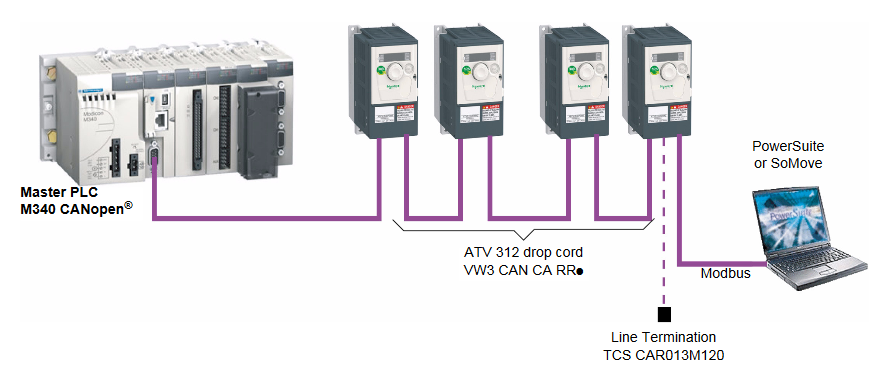
\includegraphics[scale=0.7]{comu.png}
	%\caption{Placa BME280}
	%\label{fig:BME280}
\end{figure}


\paragraph{Configuración CANopen}

\fcolorbox{red}{yellow}{imagenes. y paso a paso}\\
\\


%EL ERROR QUE TENIA CRISTIAN con ifix SE ARREGLO CON ESTO
%\url{http://www.cimexcorp.com/hasp_fix.htm}